\documentclass{ximera}

\title{Graphics, videos, and interactives}

\begin{document}
\begin{abstract}
  Embed compelling content in Ximera activities.
\end{abstract}
\maketitle

\section{Including images}

The preferred way to include graphics is with TikZ.
\begin{image}
  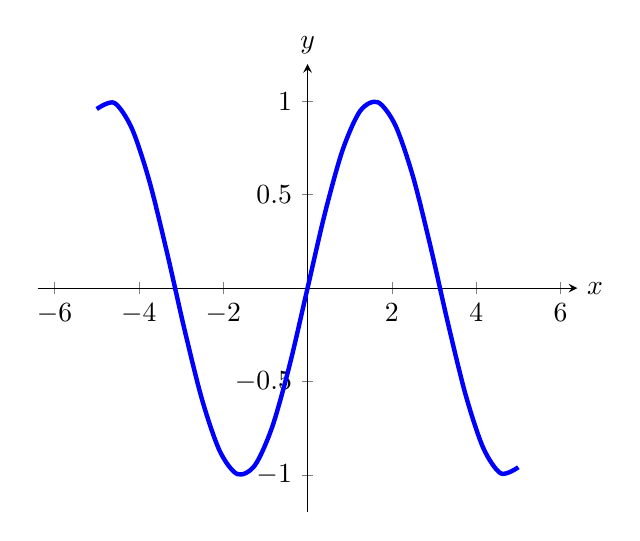
\begin{tikzpicture}
    \begin{axis}[
        xmin=-6.4,
        xmax=6.4,
        ymin=-1.2,
        ymax=1.2,
        axis lines=center,
        xlabel=$x$,
        ylabel=$y$,
        every axis y label/.style={at=(current axis.above
            origin),anchor=south},
        every axis x label/.style={at=(current axis.right of
            origin),anchor=west},
      ]
      \addplot [ultra thick, blue, smooth] {sin(deg(x))};
    \end{axis}
  \end{tikzpicture}
\end{image}

\begin{example}
\begin{verbatim}
\begin{image}
  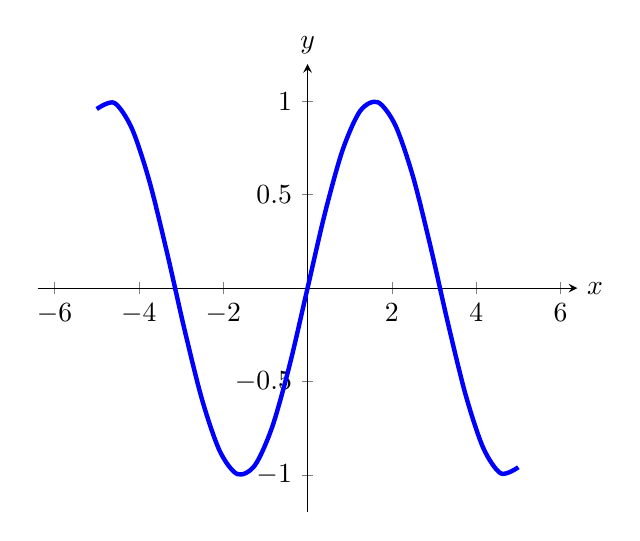
\begin{tikzpicture}
    \begin{axis}[
        xmin=-6.4,
        xmax=6.4,
        ymin=-1.2,
        ymax=1.2,
        axis lines=center,
        xlabel=$x$,
        ylabel=$y$,
        every axis y label/.style={at=(current axis.above origin),anchor=south},
        every axis x label/.style={at=(current axis.right of origin),anchor=west},
      ]
      \addplot [ultra thick, blue, smooth] {sin(deg(x))};
    \end{axis}
  \end{tikzpicture}
\end{image}
\end{verbatim}
\end{example}

\section{The graph command}

The easiest way to include an interactive graph is to use the
\verb|\graph| command. Unfortunately, the \verb|\graph| command
doesn't draw a graph in the PDF, rather, it states (in words) that a
graph is produced.
\[
  \graph{x^2}
\]
There are a number of options for the \verb|\graph| command:

\paragraph{Change viewing window}
\[
  \graph[xmin=-5,xmax=5,ymin=-5,ymax=5]{y=x^2}
\]

\paragraph{Restricting domain}
\[
  \graph{x^2 \left\{ 1 \leq x \leq 10 \right\} }
\]

\paragraph{Graphing a piecewise function}

\begin{example}
\begin{verbatim}
\[
\graph{ \sin(x)\left\{x<0\right\}, 2x\left\{ x>=0 \right\} }
\]
\end{verbatim}
\end{example}

\begin{description}
  \item[\texttt{xmin},\texttt{ymin}, \texttt{xmax},\texttt{ymax}] These set the
    size of the viewing window with \verb|\graph[xmin=-5,xmax=5,ymin=-5,ymax=5]{y=x^2}|.
\end{description}

\section{Videos}

We can embed YouTube Videos with something like
\begin{example}
\begin{verbatim}
\begin{center}
\youtube{FvgF95i0_lw}
\end{center}
\end{verbatim}
\end{example}

which would embed the video into the page, like this:
\begin{center}
  \youtube{FvgF95i0_lw}
\end{center}

\section{Desmos, Desmos 3D, and GeoGebra}

If you require further features from
\link[Desmos]{https://www.desmos.com/}, you can sign up for an account
and include your worksheets like this:
\begin{example}
\begin{verbatim}
\begin{center}
\desmos{zwywds7med}{800}{600}
\end{center}
\end{verbatim}
\end{example}
which renders as:
\begin{center}
  \desmos{zwywds7med}{800}{600}
\end{center}

The syntax for Desmos 3D is similar:
\begin{example}
\begin{verbatim}
\begin{center}
\desmosThreeD{bb4exrhrl3}{800}{600}
\end{center}
\end{verbatim}
\end{example}
Seen here:
\begin{center}
  \desmosThreeD{bb4exrhrl3}{800}{600}
\end{center}

You can also use \link[GeoGebra]{https://www.geogebra.org/}. Embed the
widget using the syntax \verb|\geogebra{ID}{width}{height}|, where ID
is the widget ID and width and height are the dimensions (in pixels)
you want the embedded widget to have.
\begin{verbatim}
  \begin{center}
  \geogebra{XC3FXUdJ}{800}{600}
  \end{center}
\end{verbatim}

\begin{center}
  \geogebra{XC3FXUdJ}{800}{600}%%https://www.geogebra.org/m/XC3FXUdJ
\end{center}

\end{document}